%!TEX TS-program = xelatex
%!TEX encoding = UTF-8 Unicode

%------------------------- IMMAGINE TIKZ
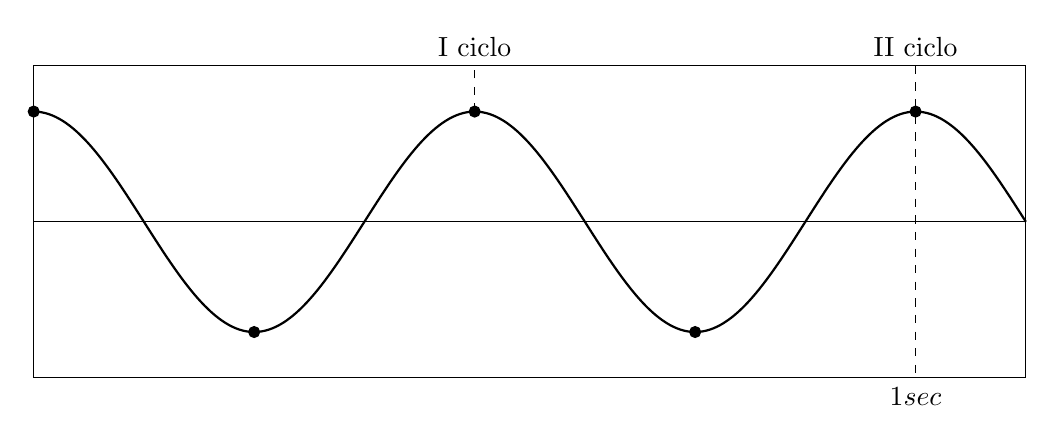
\begin{tikzpicture}[scale=.99]
  \draw[] (1.414,-2) rectangle (14.142,2);
  \draw[dashed] (12.727,2) -- (12.727,-2) node[below]{1$sec$};
  \draw[-] (1.414,0) -- (14.142,0);
       \coordinate (origin) at (0:0);
       \coordinate (A) at (45:2);
       \coordinate (-1) at (4.242,-1.414);
       \coordinate (1) at (7.071,1.414);
       \coordinate (-1b) at (9.899,-1.414);
       \coordinate (1b) at (12.727,1.414);
  \filldraw (A) circle (2pt) node[above right] {};
  \filldraw (1) circle (2pt) node[above] {};
  \filldraw (-1) circle (2pt) node[below] {};
  \filldraw (1b) circle (2pt) node[below] {};
  \filldraw (-1b) circle (2pt) node[below] {};

  \draw[dashed] (7.071,1.414) -- (7.071,2) node[above]{I ciclo};
  \draw[] (12.727,2) -- (12.727,2) node[above]{II ciclo};

  \draw[thick] (1.414,1.414) cos (2.828,0) sin (4.242,-1.414) cos (5.656, 0) sin (7.071,1.414) cos (8.485,0) sin (9.899,-1.414) cos (11.313,0) sin (12.727,1.414) cos (14.142,0);
\end{tikzpicture}
%------------------------- IMMAGINE TIKZ
